\documentclass[8pt]{beamer}
%\mode<presentation>
%{
	%\usetheme{Pittsburgh}
	%\setbeamercovered{transparent}
	%}

\usetheme{Madrid}
%\usetheme{Singapore}
%\usecolortheme{default}
%\useinnertheme{circles}
%\useoutertheme{tree}
\usefonttheme[]{serif}

%\usepackage[english,ukrainian]{babel}
%\usepackage[english]{babel}
\usepackage[OT1,T2A]{fontenc}
\usepackage[cp1251]{inputenc} % кодування документа; замість cp866nav.
\usepackage{amsfonts}

\usepackage[T1]{fontenc}
\usepackage{physics}
\usepackage{amsmath,amssymb}
\usepackage{graphicx}
\usepackage{textcomp}
\usepackage{mathtext}
\usepackage{setspace}

\usepackage{caption} % to use \caption* to skip Figure word

\usepackage{epsf}
\usepackage{amsbsy}

%\mathchardef\ordinarycolon\mathcode`\:
%\mathcode`\:=\string"8000
%\begingroup \catcode`\:=\active
%  \gdef:{\mathrel{\mathop\ordinarycolon}}
%\endgroup

%\setbeamertemplate{frametitle}{\raggedright \insertframetitle \par}

\title{Analytical determination of critical temperature}
\subtitle{for simple fluids}
\author{Roman Romanik}
%\institute{\normalsize Institute for Condensed matter physics, NAS of Ukraine}
\institute[ICMP]{\small Institute for Condensed matter physics, NAS of Ukraine}
\date{October 02, 2024}

\begin{document}
	
	%-------------------------title------------------
	
	\begin{frame}
		\titlepage
		e-mail: \url{romanik@icmp.lviv.ua}
	\end{frame}
	
	\begin{frame}
		\frametitle{Outline}
		\tableofcontents
	\end{frame}
	
	%--------------------Table of Content----------------------
	
	\section{Model Systems under Study}
	
	\begin{frame}
		\frametitle{Model Systems under Study}
		
		\begin{columns}
			\column{0.5\textwidth}
			
			-- Interaction potential: 
			\hfill
			\\
			\hfill
			
			Hard-Core + long-range attractive part
			
			(a.k.a. hard-core van der Waals fluids)
			\begin{equation*}
				\label{interaction_decomp}
				U(r_{ij}) = \Psi_{HS}(r_{ij}) + \Phi(r_{ij}),
			\end{equation*}
			
			\column{0.5\textwidth}
				\begin{figure}[htbp]
				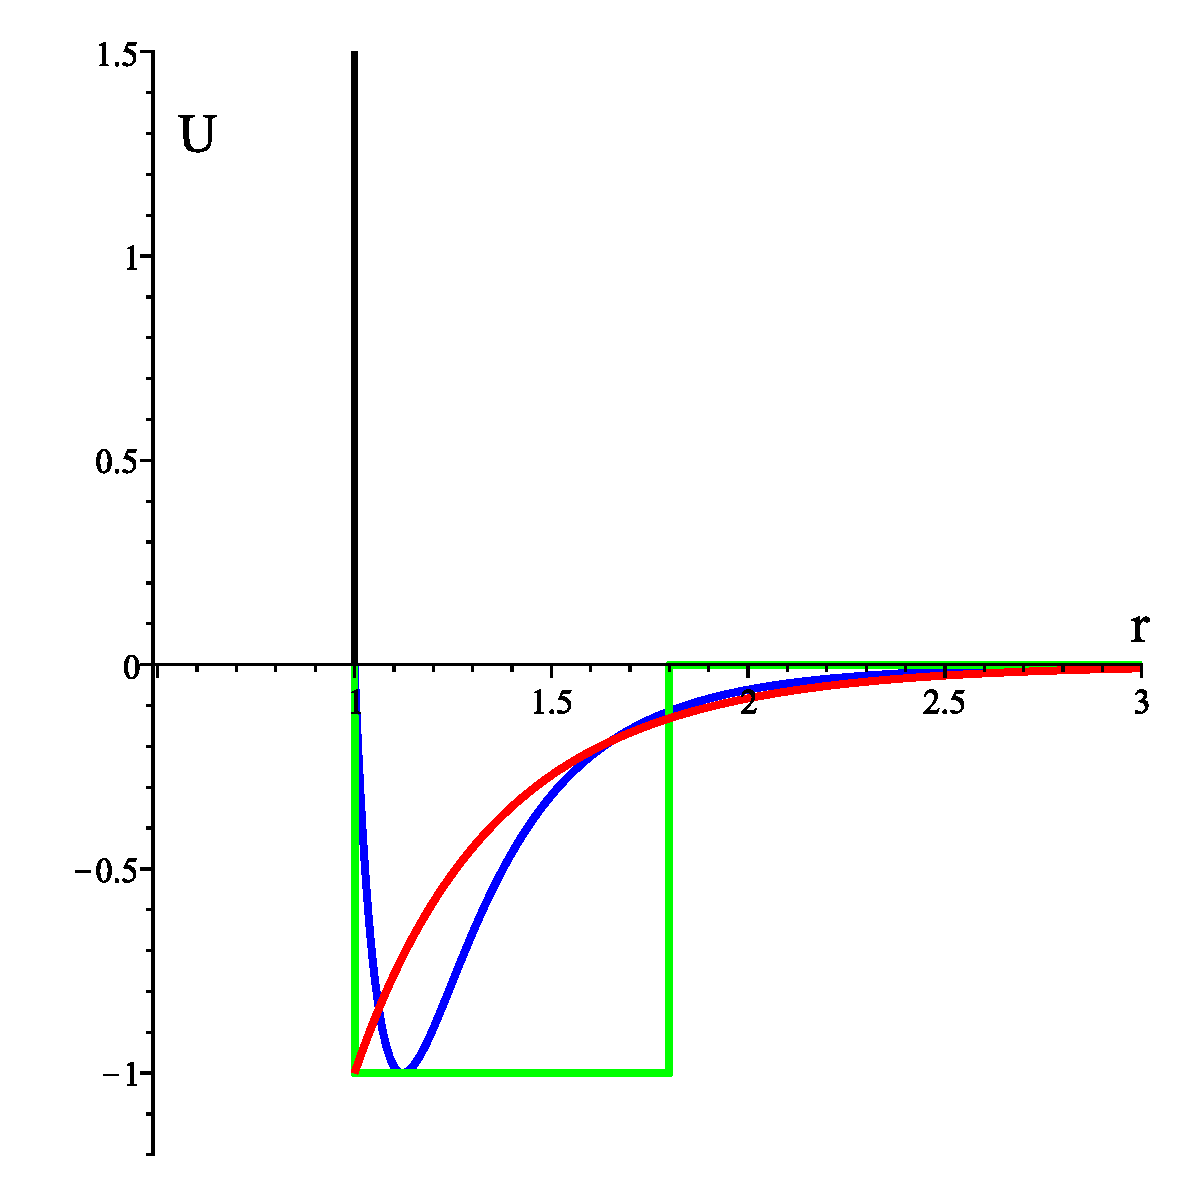
\includegraphics[width=0.9\textwidth,angle=0]{hc_vdW_fluids} \\
				\parbox{0.8\textwidth}{\caption*{Fig. 1. Typical Hard-Core van der Waals models.
				}} \hfill
			\end{figure}
		\end{columns}
		
	\end{frame}
	
	\section{Method of Collective Variables}
	\subsection{Functional of the Grand Partition Function}
	
	\begin{frame}
		\frametitle{Functional of the Grand Partition Function}
		
		\begin{equation*}
			\label{Xi_as_prod}
			\Xi = \Xi_{RS}\Xi_G\Xi_L
		\end{equation*}
		
		\begin{eqnarray*}
			\label{Xi_L_1}
			\Xi_L & \propto &
			\int \exp\left(
			\mu^* \rho_0 - \frac{1}{2} \sum_{\substack{\vb k \\ k \leq B_0}} d(k) \rho_{\vb k} \rho_{-\vb k} 
			\right.\\
			&& -\left. \frac{a_4}{4! N_0} \sum_{\substack{\vb k_1, \dotsc, \vb k_4 \\ k_i \leq B_0}} \rho_{\vb k_1} \dotsc \rho_{\vb k_4} \delta_{\vb{k}_1 + \dotsc + \vb{k}_4} \right) ({\rm d} \rho)^{N_0}
			\nonumber
		\end{eqnarray*}
		
		Notation:
		\begin{equation*}
			d(k) = a_2 + \frac{\beta\hat{\Phi}_{\vb k}}{V},
		\end{equation*}
		\begin{equation*}
			\mu^* = \beta(\mu - \mu_{RS}) + \frac{\mathfrak{m}_3}{\mathfrak{m_4}} + 
			\frac{\langle N \rangle_{RS}}{V}\beta\hat{\Phi}_0 
			\left(
			1 + \frac{\mathfrak{m}_2 \mathfrak{m}_3}{\abs{\mathfrak{m}_4}} + \frac{\mathfrak{m}_3^3}{3\mathfrak{m}_4^2}
			\right)
		\end{equation*}
		\hfill
		\\
		\hfill
		
		\textit{I.R.~Yukhnovskii, R.V.~Romanik, J. Phys. Stud., {\bf 28}(2), 2602, (2024)}
		
	\end{frame}
	
	\subsection{Layer-by-layer integration}
	
	\begin{frame}
		\frametitle{Layer-by-layer integration}
		
		\begin{columns}
			\column{0.5\textwidth}
			$B_0$ - is a cutoff parameter
			
			$N_0$ - is the number of collective variables to integrate
			\begin{equation*}
				N_0 = \frac{B_0^3}{6\pi^2}V
			\end{equation*}
			
			Parabolic approximation for the Fourier transform of long-range part of interaction
			\begin{equation*}
				\hat{\Phi}_{\vb k} = \hat{\Phi}_{0}(1 - 2b^2k^2)
			\end{equation*}
			\begin{equation*}
				2b^2 = - \frac{1}{\hat{\Phi}_{0}} \frac{\partial^2 \hat{\Phi}_{\vb k}}{\partial k^2} \bigg|_{k=0}
			\end{equation*}
			
			\column{0.5\textwidth}
			\begin{figure}[htbp]
				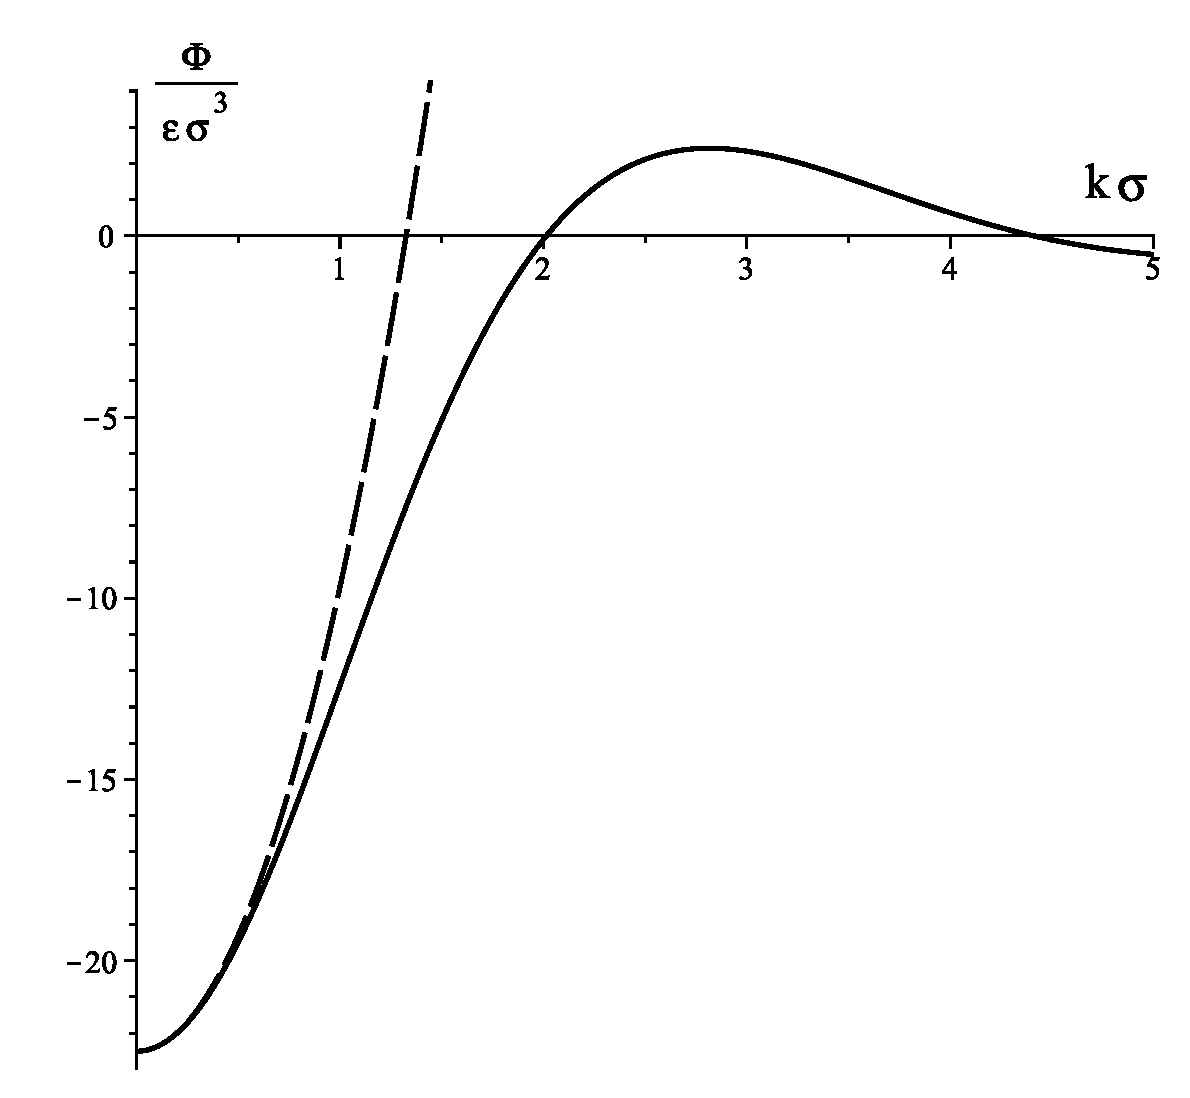
\includegraphics[width=0.9\textwidth,angle=0]{fourier_and_parabolic_potential} \\
				\parbox{0.8\textwidth}{\caption*{Fig. 2. Typical Fourier transform of the long-range part of interaction and its parabolic approximation.
				}}
			\end{figure}
		\end{columns}
	\end{frame}
	
	\begin{frame}
		\frametitle{Layer-by-layer integration}
		Integration is performed according to the method developed for the Ising model.\\
		\hfill
		
		\textbf{The main idea:} 
		\begin{itemize}
			
		\item	divide $[0, B_0]$ into sub-intervals $(B_1, B_0]$, $(B_2, B_1]$, $(B_3, B_2], \ldots$
		
		-- $B_1 = B_0/s$, $B_2 = B_1/s = B_2/s^2$, or in general $B_n = B_0/s^n$
		
		-- $s > 1$ is the renormalization group parameter
		\hfill
		\\
		\hfill
		\item $\rho_{\vb k}$ are said to belong to the first layer if $B_1 < k \leq B_0$,		
		to the second layer if $B_2 < k \leq B_1$, ..., to the $n$-th layer if $B_n < k \leq B_{n-1}$
		\hfill
		\\
		\hfill
		\item integrate iteratively, first over the CVs of the first layer, then over the second one and so on.
		
		\hfill
		
		\item replace the Fourier transform $\hat{\Phi}_{\vb k}$ with its average
		\begin{eqnarray*}
			\hat{\Phi}_{\vb k} & \rightarrow & \hat{\Phi}_{B_1, B_0}, \quad B_1 < k \leq B_0;
			\\
			& & \hat{\Phi}_{B_2, B_1}, \quad B_2 < k \leq B_1;
			\\
			& & ...
			\\
			& & \hat{\Phi}_{B_n, B_{n-1}}, \quad B_n < k \leq B_{n-1}.
		\end{eqnarray*}
		
		\end{itemize}
		
	\end{frame}
	
	\begin{frame}
		\frametitle{Layer-by-layer integration}
		
		\begin{eqnarray*}
			\Xi_L \propto \Xi_L^{(1)} & = & j_0^{-1}j_1 [Q_{f_0}]^{N_0} [Q_{\varphi_0}]^{N_1} 
			\\
			&& \times 
			\int \exp
			\left(
			\mu^*\rho_0 - \frac{1}{2} \sum_{\vb k, k \leq B_1} d_2^{(1)}(k) \rho_{\vb k} \rho_{-\vb k}
			\right.
			\nonumber \\
			&& -  
			\left.
			\frac{a_4^{(1)}}{4!N_1} \sum_{\substack{\vb k_1, \dotsc, \vb k_4 \\ k_i \leq B_1}}
			\rho_{\vb k_1} \dotsc \rho_{\vb k_4} \delta_{\vb{k}_1 + \dotsc + \vb{k}_4}
			\right) ({\rm d} \rho)^{N_1}
			\nonumber
		\end{eqnarray*}
		\hfill
		
		$N_1 = N_0 / s^3 = (B_0^3 V)/(2\pi^2 s^3)$ -- number of variables left to be integrated.
		\hfill
		\\
		\hfill
		
		$N_0 - N_1 = N_0(1-s^{-3})$ -- number of variables integrated-out.
	\end{frame}
	
	\begin{frame}
		\frametitle{Layer-by-layer integration}
		
		\textit{Yukhnovskii I.R., Romanik R., Ukr. J. Phys., {\bf 69}(9), 671, (2024)}(in print)
		
		\begin{eqnarray*}
			\label{Xi_L_1}
			\Xi &\propto & 
			\int \exp\left(
			\mu^* \rho_0 - \frac{1}{2} \sum_{\substack{\vb k \\ k \leq B_0}} d(k) \rho_{\vb k} \rho_{-\vb k} 
			\right.\\
			&& -\left. \frac{a_4}{4! N_0} \sum_{\substack{\vb k_1, \dotsc, \vb k_4 \\ k_i \leq B_0}} \rho_{\vb k_1} \dotsc \rho_{\vb k_4} \delta_{\vb{k}_1 + \dotsc + \vb{k}_4} \right) ({\rm d} \rho)^{N_0}
			\nonumber
		\end{eqnarray*}
		
		\begin{eqnarray*}
			\Longrightarrow \quad
			&\propto & j_0^{-1}j_n Q_0 Q_1 \dotsc Q_{n-1} 
			\\
			&& \times 
			\int ({\rm d} \rho)^{N_n} \exp
			\left(
			\mu^*\rho_0 - \frac{1}{2} \sum_{\vb k, k \leq B_n} d_2^{(n)}(k) \rho_{\vb k} \rho_{-\vb k}
			\right.
			\nonumber \\
			&& 
			\left.
			- \frac{a_4^{(n)}}{4!N_n} \sum_{\substack{\vb k_1, \dotsc, \vb k_4 \\ k_i \leq B_n}}
			\rho_{\vb k_1} \dotsc \rho_{\vb k_4} \delta_{\vb{k}_1 + \dotsc + \vb{k}_4}
			\right)
			\nonumber ,
		\end{eqnarray*}
	\end{frame}
	
	\begin{frame}
		\frametitle{Recurrence relations}
		
		In terms of
		\begin{eqnarray*}
			r_n & = & d_2^{(n)}(0)s^{2n},
			\\
			u_n & = & a_4^{(n)}s^{4n},
		\end{eqnarray*}
		
		The recurrence relations have the form
		\begin{eqnarray*}
			r_{n+1} & = & s^2(r_n + q) N(x_n) - s^2 q;
			\nonumber\\
			u_{n+1} & = & s u_n E(x_n).
		\end{eqnarray*}
		
		A partial solution to the RR is the fixed point
		\begin{equation*}
			r_{n+1} = r_n = r^*; \quad u_{n+1} = u_n = u^*
		\end{equation*}
		
		The particular values of the fixed point coordinates depend on the long-range interaction
		\begin{equation*}
			r^* = \frac{\beta\hat{\Phi}_0}{V} \bar{r}, 
			\qquad 
			u^* = \left(\frac{\beta\hat{\Phi}_0}{V}\right)^2 \bar{u}_0
		\end{equation*}
	\end{frame}
	
	\subsection{Coordinates of the critical point}
	
	\begin{frame}
		\frametitle{Coordinates of the critical point}
		
		\textbf{The equation for the critical temperature} $T_c^* \equiv \frac{k_{{\rm B}}T_c}{\varepsilon}$  is obtained from the condition of linearization for the RR near the fixed point
		
		\begin{equation*}
			\left(1 - \bar{r} - \sqrt{\bar{u}}R^{(0)}\right) \left(\frac{\beta\abs{\hat{\Phi}_0}}{V}\right)^2 - a_2\frac{\beta\abs{\hat{\Phi}_0}}{V} + \frac{a_4 R^{(0)}}{\sqrt{\bar{u}}} = 0
		\end{equation*}
		
		Between the two solutions, the one resulting in a positive temperature is selected
		\begin{equation*}
			\label{eq:T_c}
			T^*_c = \frac{\abs{\hat{\Phi}_0}}{\varepsilon V}
			\frac
			{2(1 - \bar{r} - R^{(0)}\sqrt{\bar{u}})}
			{a_2 + \sqrt{a_2^2 - \frac{4 a_4 R^{(0)}}{\sqrt{\bar{u}}} (1 - \bar{r} - R^{(0)}\sqrt{\bar{u}}) } }.
		\end{equation*}
		
		\textbf{The equation for the critical density} $\rho^*=\frac{\langle N \rangle}{V}\sigma^3$:
		
		[\textit{Yukhnovskii, Idzyk, Kolomiets, J. Stat. Phys., \textbf{80}, 405 (1995)}]
		\begin{equation*}
			\mathfrak{m}_3(\rho^*_c) = 0 
		\end{equation*}
		
		\begin{eqnarray*}
			\rho^*_c & = & 0.2491 \quad \text{in Carnahan-Starling approximation}
			\\
			\rho^*_c & = & 0.2457 \quad \text{in Percus-Yevick approximation}
		\end{eqnarray*}
	\end{frame}
	
	\section{Results}
	
	\begin{frame}
		\frametitle{Hard-Core Square-well fluid}
		
		\begin{columns}
			\column{0.5\textwidth}
			Square-well potential: 
			\begin{equation*}
				\label{def:sw}
				\phi^{SW}(r) = \left\{
				\begin{array}{llll}
					\infty, & r\leq \sigma,
					\\
					-\varepsilon, & \sigma < r \leq \lambda\sigma,
					\\
					0, & r > \sigma.
				\end{array}
				\right.
			\end{equation*}
			
			There are several options for defining long-range interaction for $r\leq \sigma$:
			\hfill
			\\
			\hfill
			
			-- setting the potential to zero:			
			\begin{equation*}
				\Phi(r) = \left\{
				\begin{array}{cc}
					0, & r \leq \sigma, 
					\\
					\phi^{SW}(r), & r > \sigma;
				\end{array}
				\right.
			\end{equation*}
			
			-- applying the Weeks-Chandler-Andersen regularization:			
			\begin{equation*}
				\Phi(r) = \left\{
				\begin{array}{cc}
					-\varepsilon, & r \leq \sigma, 
					\\
					\phi^{SW}(r), & r > \sigma.
				\end{array}
				\right.
			\end{equation*}
			
			\textit{Weeks, Chandler, Andersen, J. Chem. Phys. \textbf{54}, 5237 (1971)}
			
			\column{0.5\textwidth}
			\begin{figure}[htbp]
				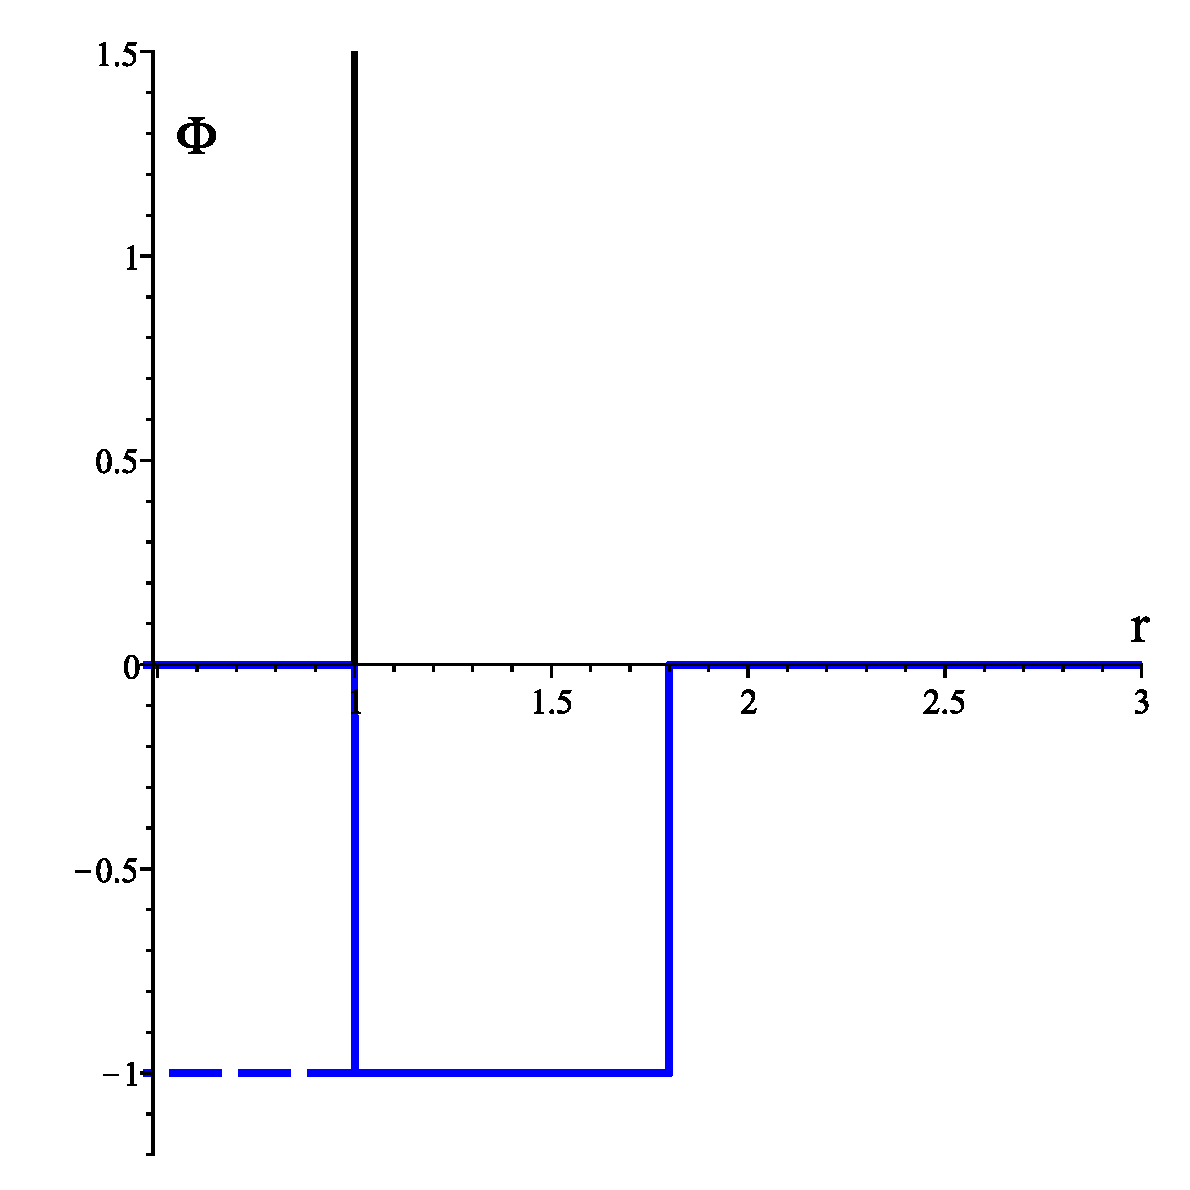
\includegraphics[width=0.9\textwidth,angle=0]{hcsw} \\
				\parbox{0.8\textwidth}{\caption*{Fig. 3. Different regularizations for the square-well potential.
				}}
			\end{figure}
			
		\end{columns}
		
	\end{frame}
	
	\begin{frame}
		\frametitle{Hard-Core Square-well fluid}
		
		\begin{columns}
			\column{0.5\textwidth}
			Square-well potential: 
			\begin{equation*}
				\label{def:sw}
				\phi^{SW}(r) = \left\{
				\begin{array}{llll}
					\infty, & r\leq \sigma,
					\\
					-\varepsilon, & \sigma < r \leq \lambda\sigma,
					\\
					0, & r > \sigma.
				\end{array}
				\right.
			\end{equation*}
			
			There are several options for defining long-range interaction for $r\leq \sigma$:
			\hfill
			\\
			\hfill
			
			-- setting the potential to zero:			
			\begin{equation*}
				\Phi(r) = \left\{
				\begin{array}{cc}
					0, & r \leq \sigma, 
					\\
					\phi^{SW}(r), & r > \sigma;
				\end{array}
				\right.
			\end{equation*}
			
			-- applying the Weeks-Chandler-Andersen regularization:			
			\begin{equation*}
				\Phi(r) = \left\{
				\begin{array}{cc}
					-\varepsilon, & r \leq \sigma, 
					\\
					\phi^{SW}(r), & r > \sigma.
				\end{array}
				\right.
			\end{equation*}
			
			\textit{Weeks, Chandler, Andersen, J. Chem. Phys. \textbf{54}, 5237 (1971)}
			
			\column{0.5\textwidth}
			\begin{figure}[htbp]
				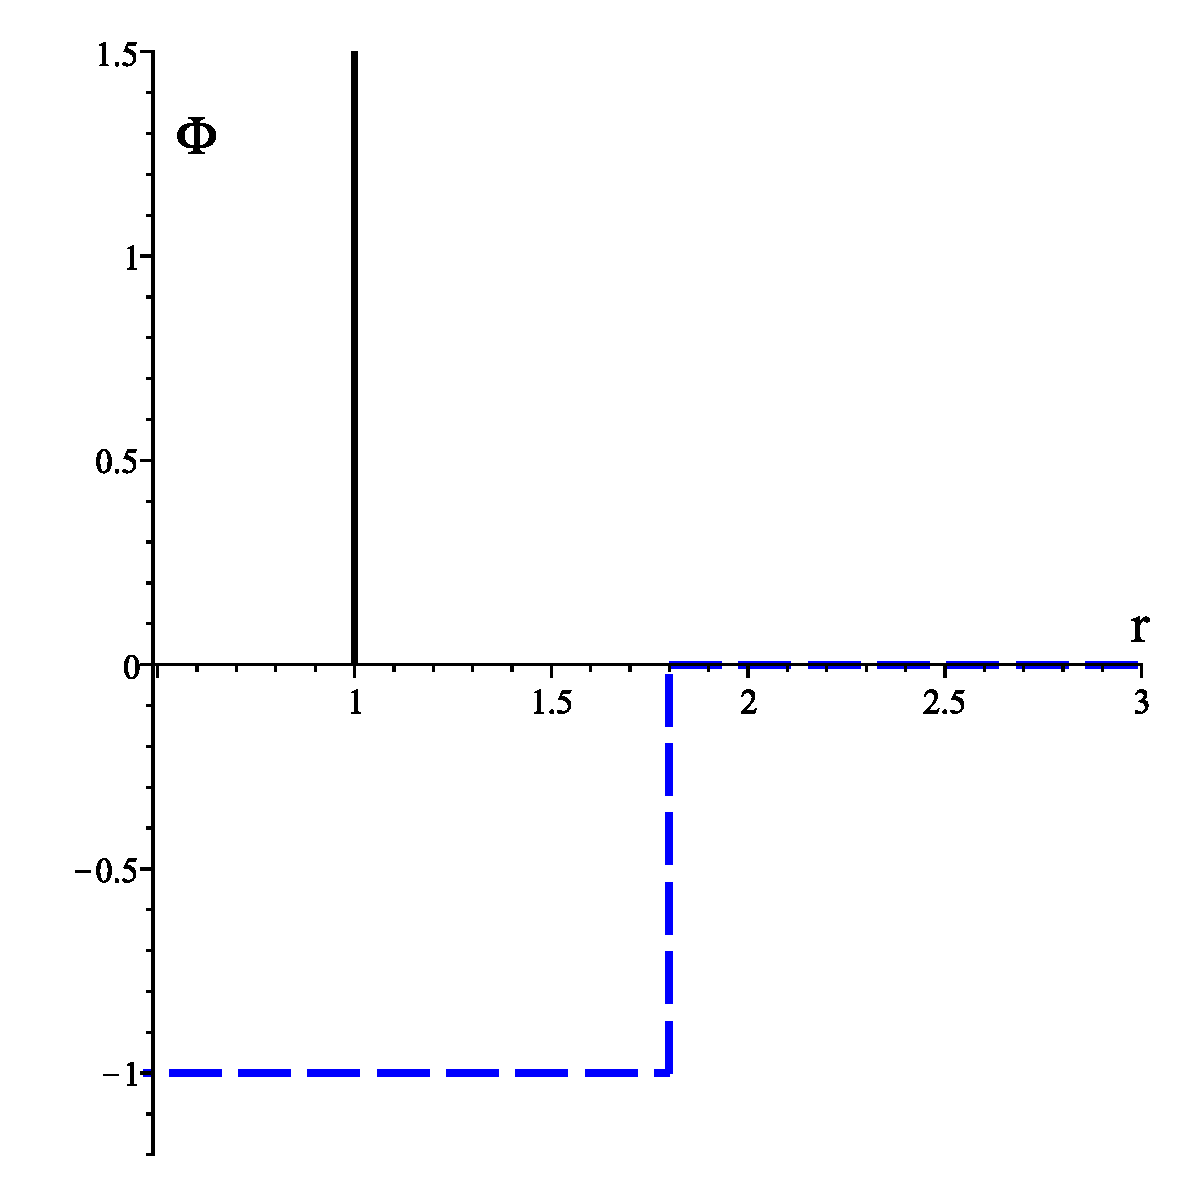
\includegraphics[width=0.9\textwidth,angle=0]{hcsw_wca} \\
				\parbox{0.8\textwidth}{\caption*{Fig. 3. Different regularizations for the square-well potential.
				}}
			\end{figure}
						
		\end{columns}
		
	\end{frame}
	
	\iffalse
	\begin{frame}
		\frametitle{Hard-Core Square-well fluid}
		
		\begin{columns}
			\column{0.5\textwidth}
			Square-well potential: 
			\begin{equation*}
				\label{def:sw}
				\phi^{SW}(r) = \left\{
				\begin{array}{llll}
					\infty, & r\leq \sigma,
					\\
					-\varepsilon, & \sigma < r \leq \lambda\sigma,
					\\
					0, & r > \sigma.
				\end{array}
				\right.
			\end{equation*}
			
			There are several options for defining long-range interaction for $r\leq \sigma$:
			\hfill
			\\
			\hfill
			
			-- setting the potential to zero:			
			\begin{equation*}
				\Phi(r) = \left\{
				\begin{array}{cc}
					0, & r \leq \sigma, 
					\\
					\phi^{SW}(r), & r > \sigma;
				\end{array}
				\right.
			\end{equation*}
			
			-- applying the Weeks-Chandler-Andersen regularization:			
			\begin{equation*}
				\Phi(r) = \left\{
				\begin{array}{cc}
					-\varepsilon, & r \leq \sigma, 
					\\
					\phi^{SW}(r), & r > \sigma.
				\end{array}
				\right.
			\end{equation*}
			
			\textit{Weeks, Chandler, Andersen, J. Chem. Phys. \textbf{54}, 5237 (1971)}
			
			\column{0.5\textwidth}
			
			\begin{table}[h]
				\noindent\caption{Critical temperature of the HC square-well fluid for different values of $\lambda$.}\vskip3mm\tabcolsep4.5pt
				\begin{tabular}{|c|c|c|c|}
					\hline
					\multicolumn{4}{|c|}{Square-well}\\
					\hline
					$\lambda$ & $T_c^*$& $T_c^*$ (WCA) & $T_c^*$ [1] \\
					\hline
					1.25 & 0.35 & 0.78 & 0.75 \\
					1.50 & 0.84 & 1.26 & 1.25 \\
					1.75 & 1.52 & 1.92 & 1.88 \\
					2.00 & 2.41 & 2.79 & 2.72 \\
					\hline
				\end{tabular}
				\label{tab:sw_temp_cr}
			\end{table}
			
			[1] \textit{Krejci, Nezbeda, Fluid Phase Equilib. \textbf{314}, 156 (2012)}
			
		\end{columns}
		
	\end{frame}
	\fi
	
	\begin{frame}
		\frametitle{Hard-Core Square-well fluid}
		
		\begin{columns}
			\column{0.5\textwidth}
			\begin{figure}[htbp]
				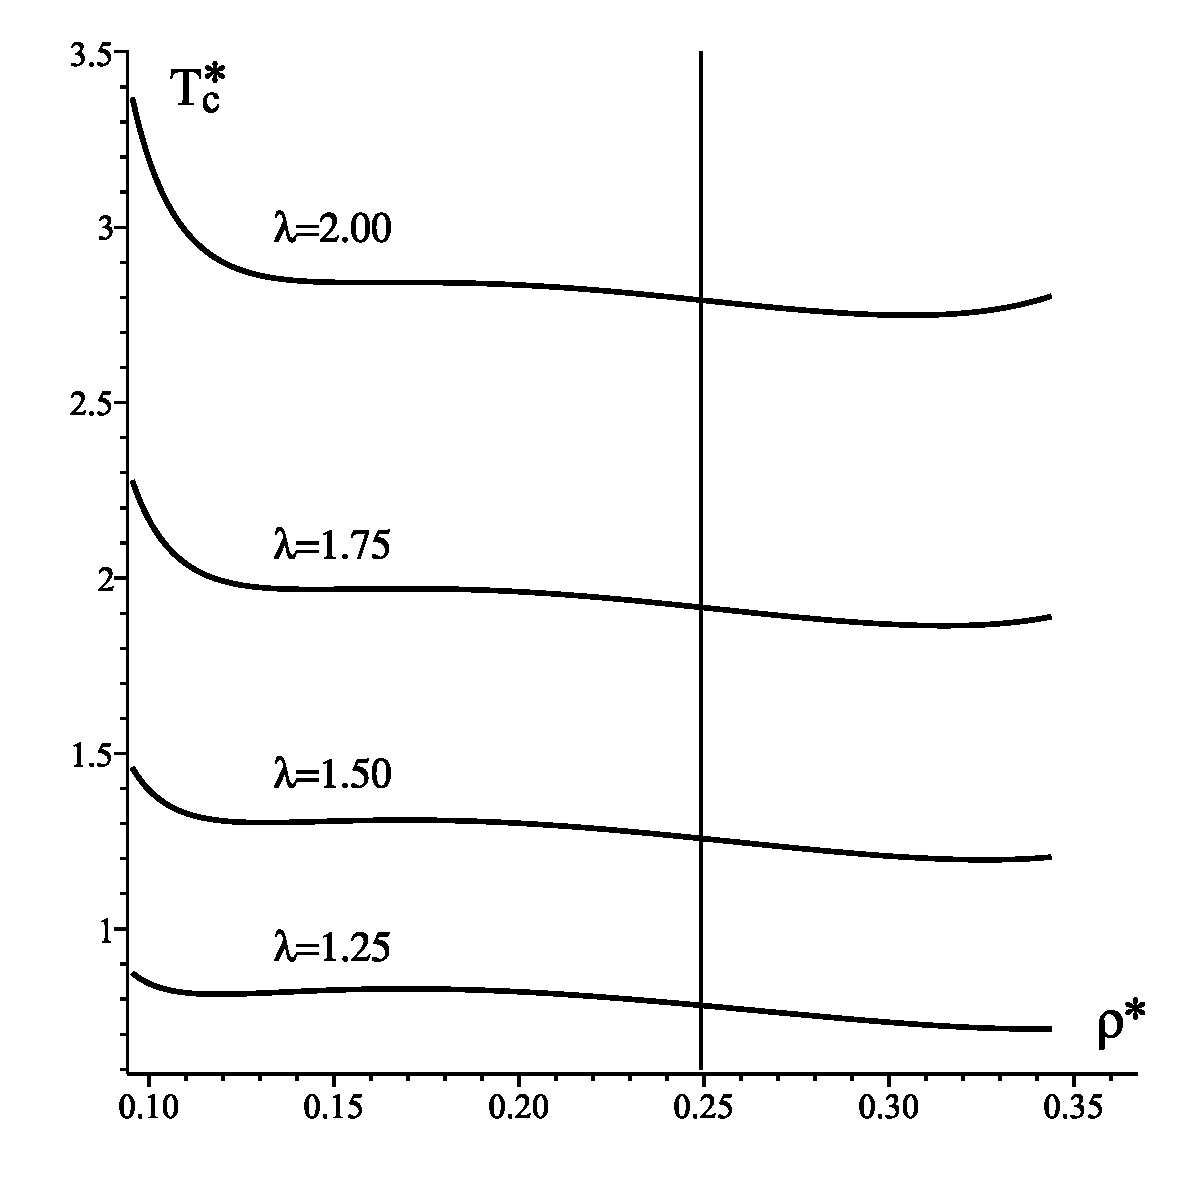
\includegraphics[width=0.9\textwidth,angle=0]{cp_coord} \\
				\parbox{0.8\textwidth}{\caption*{Fig. 4. The critical point coordinates for different values of parameter $\lambda$.
				}}
			\end{figure}
			
			\textit{Yukhnovskii, Romanik, Ukr. J. Phys., {\bf 69}(9), 671, (2024)}(in print)
			
			\column{0.5\textwidth}
			
			\begin{table}[h]
				\noindent\caption{Critical temperature of the HC square-well fluid for different values of $\lambda$.}\vskip3mm\tabcolsep4.5pt
				\begin{tabular}{|c|c|c|c|}
					\hline
					\multicolumn{4}{|c|}{Square-well}\\
					\hline
					$\lambda$ & $T_c^*$& $T_c^*$ (WCA) & $T_c^*$ [1] \\
					\hline
					1.25 & 0.35 & 0.78 & 0.75 \\
					1.50 & 0.84 & 1.26 & 1.25 \\
					1.75 & 1.52 & 1.92 & 1.88 \\
					2.00 & 2.41 & 2.79 & 2.72 \\
					\hline
				\end{tabular}
			\end{table}
			
			[1] \textit{Krejci, Nezbeda, Fluid Phase Equilib. \textbf{314}, 156 (2012)}
			
		\end{columns}
		
	\end{frame}
	
	\begin{frame}
		\frametitle{Hard-Core Yukawa fluid}
		
		\begin{columns}
			\begin{column}{0.5\textwidth}
				Yukawa potential:
				\begin{equation*}
					\label{def:yukawa}
					\phi^Y(r) = -\frac{\varepsilon \sigma}{r} \exp[-\lambda(r/\sigma - 1)].
				\end{equation*}
				
				Long-range interaction regularization for $r \leq \sigma$:
				\hfill
				\\
				\hfill
				
				-- setting the potential to zero:
				\begin{equation*}
					\Phi(r) = \left\{
					\begin{array}{ll}
						0, & r \leq \sigma 
						\\
						\phi^Y(r), & r > \sigma.
					\end{array}
					\right.
				\end{equation*}
				
				-- Applying the WCA regularization:
				\begin{equation*}
					\Phi(r) = \left\{
					\begin{array}{ll}
						-\varepsilon, & r \leq \sigma 
						\\
						\phi^Y(r), & r > \sigma.
					\end{array}
					\right.
				\end{equation*}
			\end{column}
			
			\begin{column}{0.5\textwidth}
				\begin{figure}[htbp]
					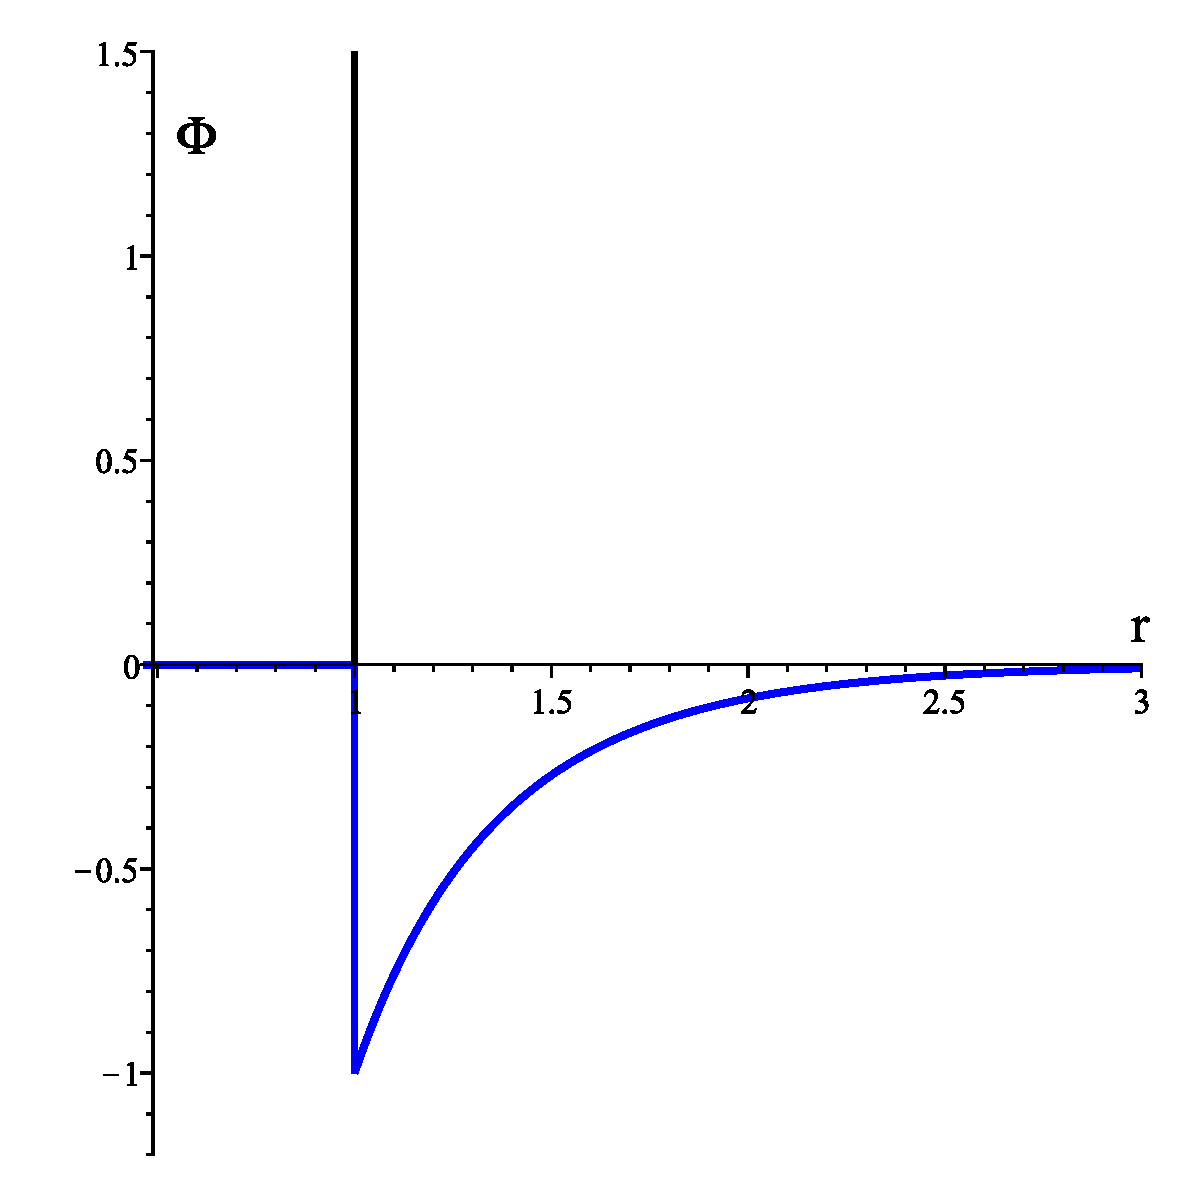
\includegraphics[width=0.9\textwidth,angle=0]{hcy} \\
					\parbox{0.8\textwidth}{\caption*{Fig. 5. Different regularizations for the hard-core Yukawa potential.
					}}
				\end{figure}
			\end{column}
			
		\end{columns}
		
	\end{frame}
	
	\begin{frame}
		\frametitle{Hard-Core Yukawa fluid}
		
		\begin{columns}
			\begin{column}{0.5\textwidth}
				Yukawa potential:
				\begin{equation*}
					\label{def:yukawa}
					\phi^Y(r) = -\frac{\varepsilon \sigma}{r} \exp[-\lambda(r/\sigma - 1)].
				\end{equation*}
				
				Long-range interaction regularization for $r \leq \sigma$:
				\hfill
				\\
				\hfill
				
				-- setting the potential to zero:
				\begin{equation*}
					\Phi(r) = \left\{
					\begin{array}{ll}
						0, & r \leq \sigma 
						\\
						\phi^Y(r), & r > \sigma.
					\end{array}
					\right.
				\end{equation*}
				
				-- Applying the WCA regularization:
				\begin{equation*}
					\Phi(r) = \left\{
					\begin{array}{ll}
						-\varepsilon, & r \leq \sigma 
						\\
						\phi^Y(r), & r > \sigma.
					\end{array}
					\right.
				\end{equation*}
			\end{column}
			
			\begin{column}{0.5\textwidth}
				\begin{figure}[htbp]
					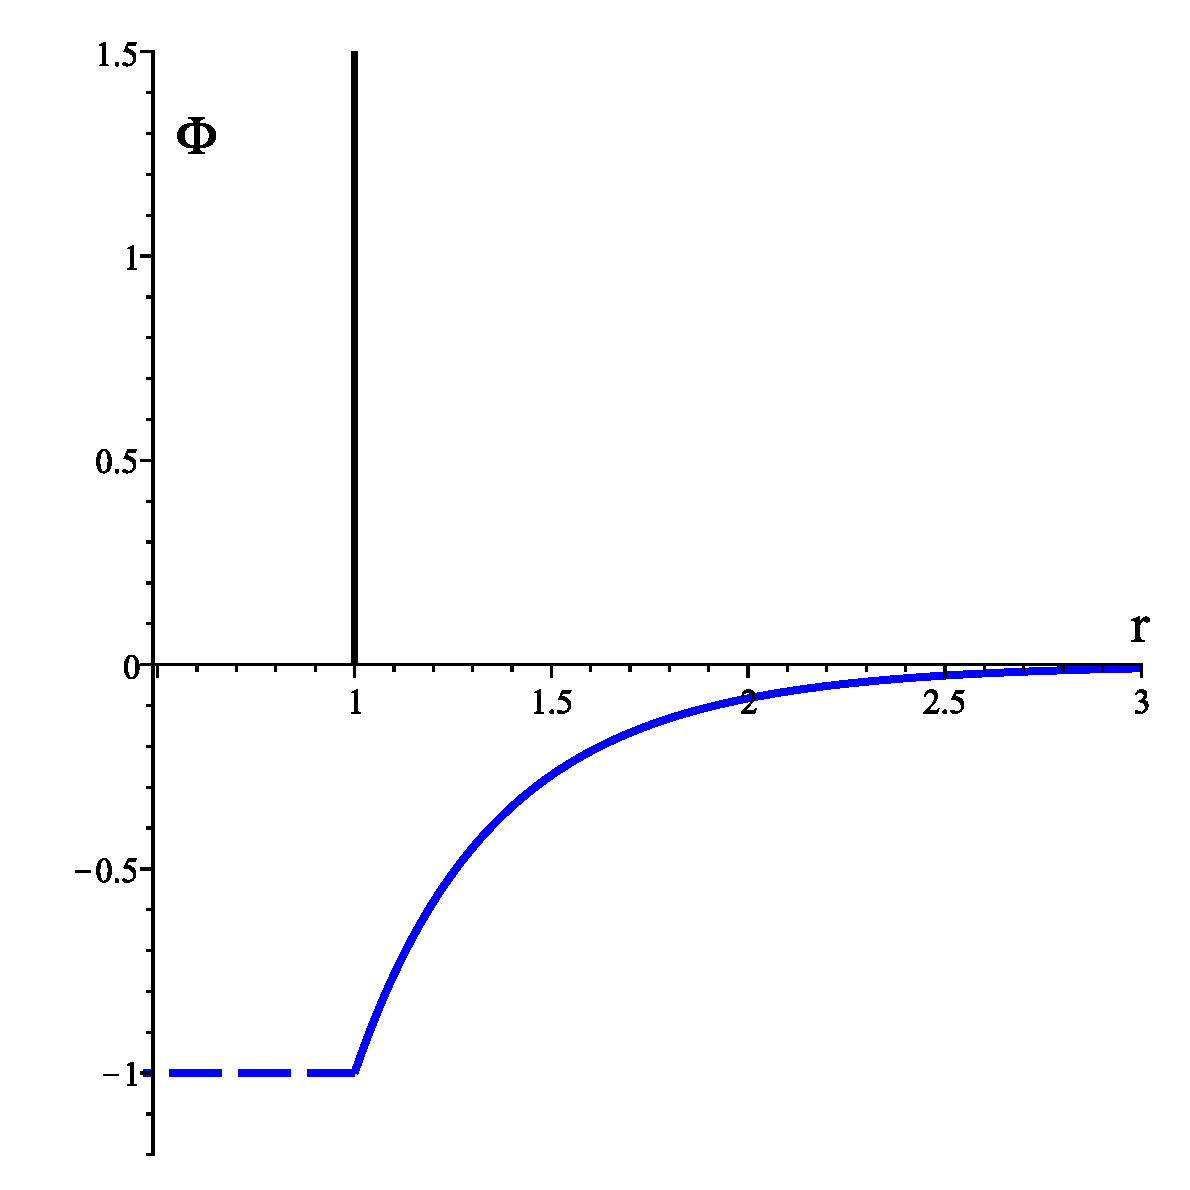
\includegraphics[width=0.9\textwidth,angle=0]{hcy_wca} \\
					\parbox{0.8\textwidth}{\caption*{Fig. 5. Different regularizations for the hard-core Yukawa potential.
					}}
				\end{figure}
			\end{column}
			
		\end{columns}
		
	\end{frame}
	
	\begin{frame}
		\frametitle{Hard-Core Yukawa fluid}
		
		\begin{columns}
			\begin{column}{0.5\textwidth}
				Yukawa potential:
				\begin{equation*}
					\label{def:yukawa}
					\phi^Y(r) = -\frac{\varepsilon \sigma}{r} \exp[-\lambda(r/\sigma - 1)].
				\end{equation*}
				
				Long-range interaction regularization for $r \leq \sigma$:
				\hfill
				\\
				\hfill
				
				-- setting the potential to zero:
				\begin{equation*}
					\Phi(r) = \left\{
					\begin{array}{ll}
						0, & r \leq \sigma 
						\\
						\phi^Y(r), & r > \sigma.
					\end{array}
					\right.
				\end{equation*}
				
				-- Applying the WCA regularization:
				\begin{equation*}
					\Phi(r) = \left\{
					\begin{array}{ll}
						-\varepsilon, & r \leq \sigma 
						\\
						\phi^Y(r), & r > \sigma.
					\end{array}
					\right.
				\end{equation*}
			\end{column}
			
			\begin{column}{0.5\textwidth}
				
				\begin{table}[h]
					\noindent\caption{Critical temperature of the HC Yukawa fluid for different values of $\lambda$.}\vskip3mm\tabcolsep4.5pt
					\begin{tabular}{|c|c|c|c|}
						%\begin{tabular}{cccccccccc}
						\hline
						\multicolumn{4}{|c|}{HC Yukawa}\\
						\hline
						$\lambda$ & $T_c^*$ & $T_c^*$ (WCA)& $T_c^*$ [2] \\
						\hline
						0.5 & 6.15 & 7.24 & 7.009 \\
						1.0 & 2.07 & 2.69 & 2.486 \\
						1.5 & 1.16 & 1.69 & 1.634 \\
						1.8 & 0.90 & 1.41 & 1.228 \\
						2.0 & 0.79 & 1.28 & 1.031 \\
						2.5 & 0.59 & 1.07 & 0.836 \\
						3.0 & 0.47 & 0.94 & 0.722 \\
						\hline
					\end{tabular}
					\label{tab:yukawa_temp_cr}
				\end{table}
				
				[2] \textit{El Mendoub, Wax, Jakse, J. Chem. Phys. \textbf{132}, 164503 (2010)}
			\end{column}
						
		\end{columns}
						
	\end{frame}
	
	\begin{frame}
		\frametitle{Hard-Core Lennard-Jones fluid}
		
		\begin{columns}
			\begin{column}{0.55\textwidth}
				The Hard-Core Lennard-Jones potential
				\begin{equation*}
					\phi^{LJ}(r) = \left\{
					\begin{array}{llll}
						\infty, & r\leq \sigma,
						\\
						-\varepsilon, & \sigma < r \leq r_{\rm m}, 
						\\
						4\varepsilon \left[(\sigma/r)^{12} - (\sigma/r)^6\right], & r > r_{\rm m},
					\end{array}
					\right.
				\end{equation*}
				where $r_{\rm m}=2^{1/6}\sigma$.
				
				\textit{Sowers, Sandler, Fluid Phase Equilib \textbf{63}, 1 (1991)}
				\hfill
				\\
				\hfill
				
				The WCA regularization for the long-range interaction:
				\begin{equation*}
					\Phi(r) = \left\{
					\begin{array}{ll}
						-\varepsilon, & r \leq r_{\rm m},
						\\
						4\varepsilon \left[(\sigma/r)^{12} - (\sigma/r)^6\right], & r > r_{\rm m}.
					\end{array}	
					\right.
				\end{equation*}
			\end{column}
			
			\begin{column}{0.4\textwidth}
				
				\begin{figure}[htbp]
					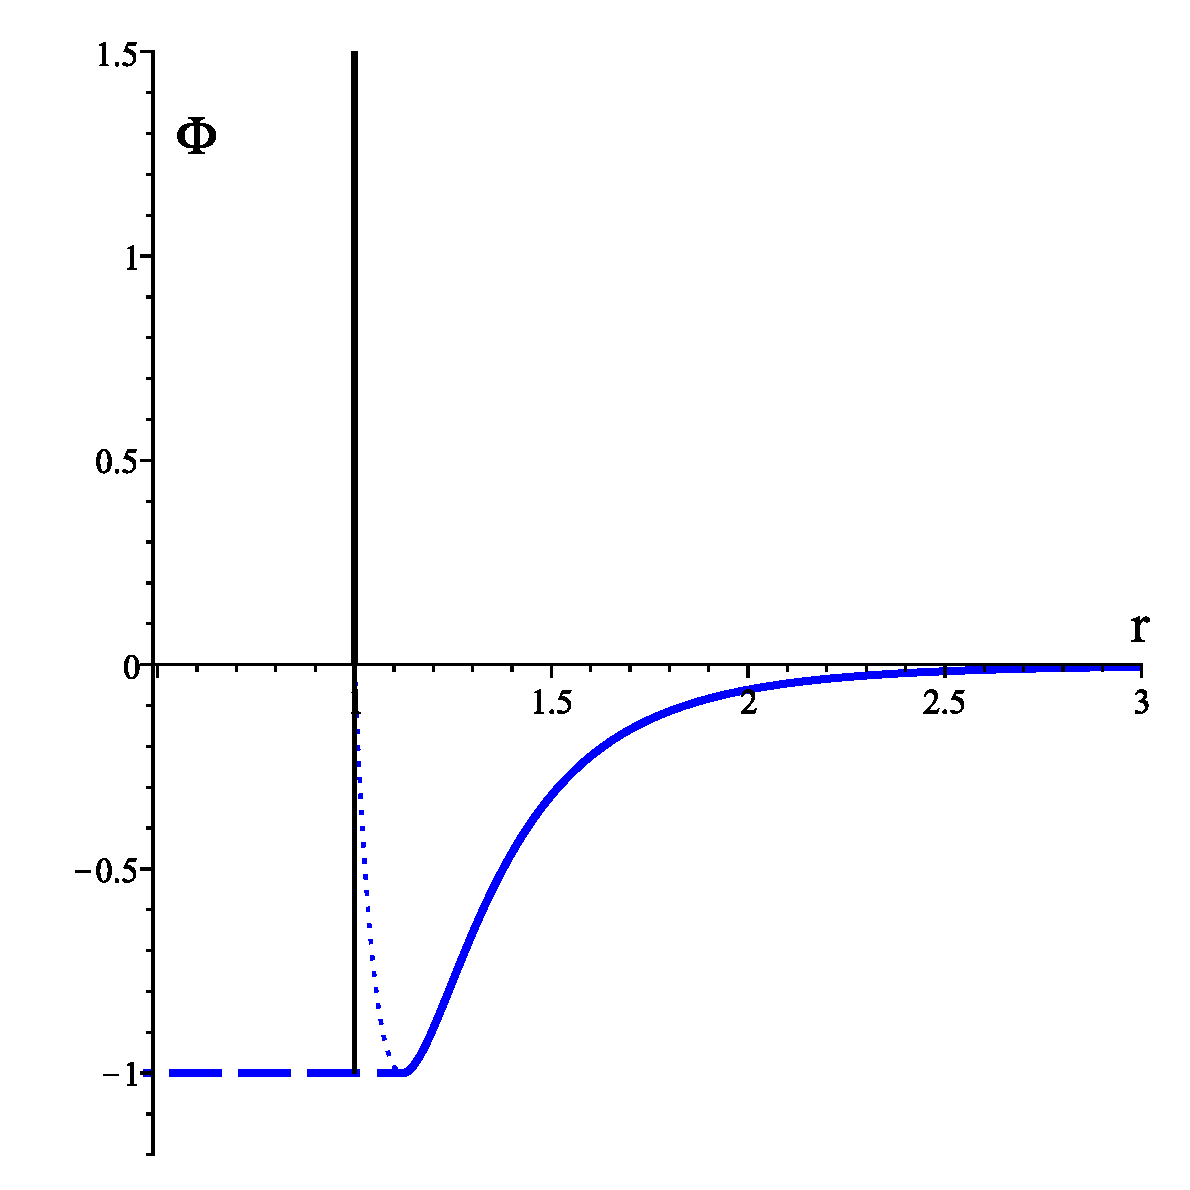
\includegraphics[width=0.9\textwidth,angle=0]{hclj_wca} \\
					\parbox{0.8\textwidth}{\caption*{Fig. 5. Different regularizations for the hard-core Lennard-Jones potential.
				}}
				\end{figure}				
			\end{column}
			
		\end{columns}
		
	\end{frame}
	
	
	\begin{frame}
		\frametitle{Hard-Core Lennard-Jones fluid}
		
		\begin{columns}
			\begin{column}{0.55\textwidth}
				The Hard-Core Lennard-Jones potential
				\begin{equation*}
					\phi^{LJ}(r) = \left\{
					\begin{array}{llll}
						\infty, & r\leq \sigma,
						\\
						-\varepsilon, & \sigma < r \leq r_{\rm m}, 
						\\
						4\varepsilon \left[(\sigma/r)^{12} - (\sigma/r)^6\right], & r > r_{\rm m},
					\end{array}
					\right.
				\end{equation*}
				where $r_{\rm m}=2^{1/6}\sigma$.
				
				\textit{Sowers, Sandler, Fluid Phase Equilib \textbf{63}, 1 (1991)}
				\hfill
				\\
				\hfill
				
				The WCA regularization for the long-range interaction:
				\begin{equation*}
					\Phi(r) = \left\{
					\begin{array}{ll}
						-\varepsilon, & r \leq r_{\rm m},
						\\
						4\varepsilon \left[(\sigma/r)^{12} - (\sigma/r)^6\right], & r > r_{\rm m}.
					\end{array}	
					\right.
				\end{equation*}
			\end{column}
			
			\begin{column}{0.4\textwidth}
				
				\begin{table}[h]
					\noindent\caption{Critical temperature of the HC Lennard-Jones fluid}\vskip3mm\tabcolsep4.5pt
					\begin{tabular}{|c|c|}
						\hline
						\multicolumn{2}{|c|}{HC Lennard-Jones}\\
						\hline
						$T_c^*$ (WCA) & $T_c^*$ [3] \\
						\hline
						1.43 & 1.375 \\
						\hline
					\end{tabular}
					\label{tab:lj_temp_cr}
				\end{table}
				
				[3] \textit{Sowers, Sandler, Fluid Phase Equilib. \textbf{63}, 1 (1991)}
				
			\end{column}
			
		\end{columns}
		
	\end{frame}
	
	\begin{frame}
		\frametitle{Hard-Core Morse fluid}
		
		\begin{columns}
			\begin{column}{0.5\textwidth}
				Morse potential:
				\begin{equation*}
					%\label{def:morse}
					\phi^M(r) = \varepsilon \{{\rm e}^{-2(r-R_0)/\alpha}-2{\rm e}^{-(r-R_0)/\alpha}\}.
				\end{equation*}
				
				Long-range interaction regularization for $r \leq \sigma$:
				\begin{equation*}
					\Phi(r) = \left\{
					\begin{array}{ll}
						0, & r \leq \sigma 
						\\
						\phi^M(r), & r > \sigma.
					\end{array}
					\right.
				\end{equation*}
								
			\end{column}
			
			\begin{column}{0.5\textwidth}
				\begin{figure}[htbp]
					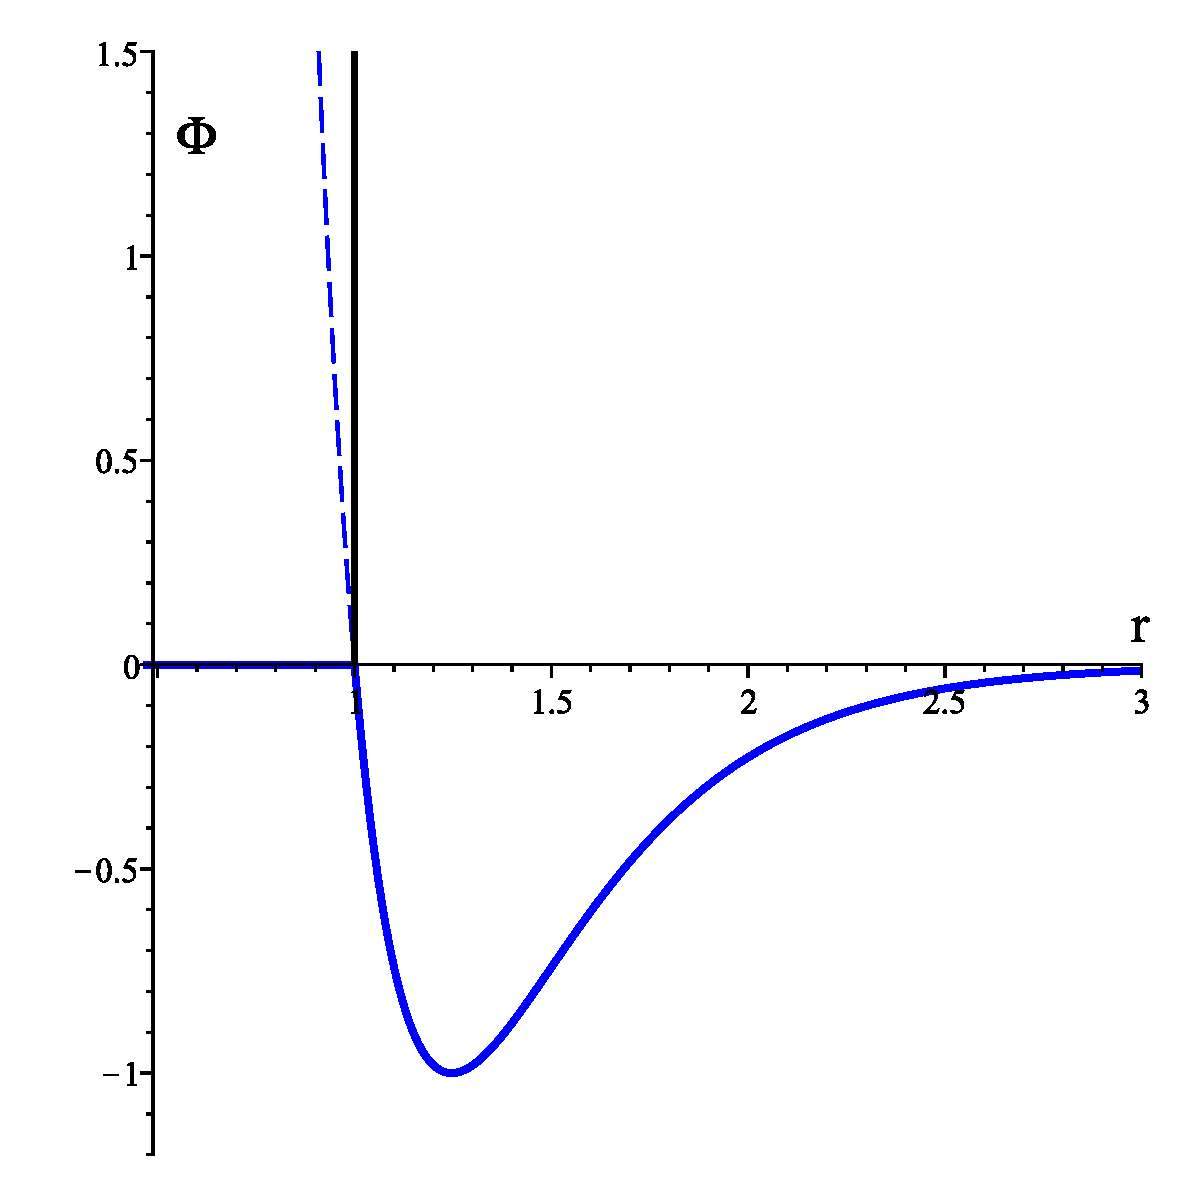
\includegraphics[width=0.9\textwidth,angle=0]{hcmorse} \\
					\parbox{0.8\textwidth}{\caption*{Fig. 5. Different regularizations for the hard-core Morse potential.
					}}
				\end{figure}
				
			\end{column}
		\end{columns}
		
	\end{frame}
	
	\begin{frame}
		\frametitle{Hard-Core Morse fluid}
		
		\begin{columns}
			\begin{column}{0.5\textwidth}
				Morse potential:
				\begin{equation*}
					%\label{def:morse}
					\phi^M(r) = \varepsilon \{{\rm e}^{-2(r-R_0)/\alpha}-2{\rm e}^{-(r-R_0)/\alpha}\}.
				\end{equation*}
				
				Long-range interaction regularization for $r \leq \sigma$:
				\begin{equation*}
					\Phi(r) = \left\{
					\begin{array}{ll}
						0, & r \leq \sigma 
						\\
						\phi^M(r), & r > \sigma.
					\end{array}
					\right.
				\end{equation*}
				
				
			\end{column}
			
			\begin{column}{0.5\textwidth}
				
				\begin{table}[h]
					\noindent\caption{Critical temperature of the HC Morse fluid for different values of $R_0/\alpha$.}\vskip3mm\tabcolsep4.5pt
					\begin{tabular}{|c|c|}
						\hline
						\multicolumn{2}{|c|}{HC Morse} \\
						\hline
						$R_0/\alpha$ \quad & $T_c^*$ \\
						\hline
						2.0  & 4.2852 \\
						2.5  & 2.1593 \\
						3.0  & 1.3418 \\
						3.5  & 0.9396 \\
						4.0  & 0.7096 \\
						4.5  & 0.5641 \\
						5.0  & 0.4652 \\
						\hline
					\end{tabular}
					\label{tab:morse_temp_cr}
				\end{table}
			\end{column}
		\end{columns}
		
	\end{frame}
	
	\section{Additional discussion}
	
	\subsection{When does a critical point disappear?}
	
	\begin{frame}
		\frametitle{When does a critical point disappear?}
		
		\begin{columns}
			\begin{column}{0.5\textwidth}
				\begin{figure}[htbp]
					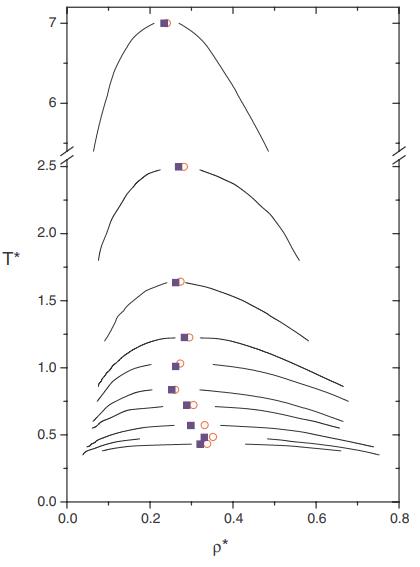
\includegraphics[width=0.65\textwidth,angle=0]{limit_cp_spinodals} \\
					\parbox{1.0\textwidth}{\caption*{Fig. 2. Spinodal lines for HC Yukawa fluid for $\lambda = 0.5,$ $\lambda = 1.0,$ $\lambda = 1.5,$ $\lambda = 1.8,$ $\lambda = 2.0,$ $\lambda = 2.5,$ $\lambda = 3.0,$ $\lambda = 4.0,$ $\lambda = 5.0,$ $\lambda = 6.0$.
					}}
				\end{figure}
				
				\textit{El Mendoub, Wax, Jakse, J. Chem. Phys. \textbf{132}, 164503 (2010)}
			\end{column}
			
			\begin{column}{0.5\textwidth}
				\begin{figure}[htbp]
					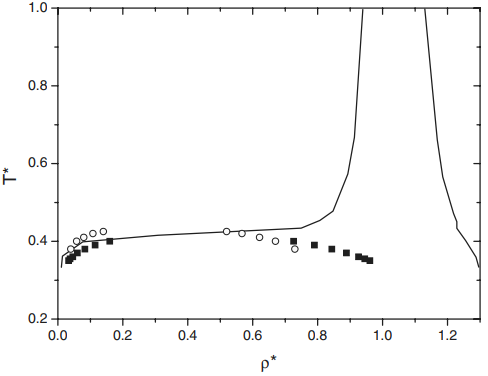
\includegraphics[width=0.75\textwidth,angle=0]{limit_cp} \\
					\parbox{1.0\textwidth}{\caption*{Fig. 2. Limiting case when a critical point disappears for the HC Yukawa fluid. Fluid-solid binodal [1] (solid line) and liquid-vapor binodal [2] (full squares) for $\lambda=7$. Liquid-vapor binodal [3] (open circles) for $\lambda = 6$.
					}}
				\end{figure}
				
				[1] \textit{Dijkstra, Phys. Rev. E \textbf{66}, 021402 (2002)}
				[2] \textit{Duda, Romero-Martinez, Orea, J. Chem. Phys. \textbf{126}, 224510 (2007)}
				
				[3]\textit{El Mendoub, Wax, Jakse, J. Chem. Phys. \textbf{132}, 164503 (2010)}
			\end{column}
			
		\end{columns}
		
	\end{frame}
	
	\begin{frame}
		\frametitle{Critical density}
		
		\begin{eqnarray*}
			\rho^*_c = 0.2491 & \quad (\eta_c = 0.13044) & \quad \text{in Carnahan-Starling approximation}
			\\
			\rho^*_c = 0.2457 & & \quad \text{in Percus-Yevick approximation}
		\end{eqnarray*}
		
		\uncover<2-> {
			Exactly these values are mentioned in [\textit{Trokhymchuk, Melnyk, Holovko, Nezbeda, J.Mol.Liq. \textbf{228}, 194 (2017)}] for Sutherland fluid with HC reference.
		}
		
		\begin{table}[h]
			\noindent\caption{Critical density of some HC van der Waals fluids.}\tabcolsep4.5pt
			\begin{tabular}{|c|c|c|c|c|}
				\hline
				\multicolumn{2}{|c|}{Square-well}& \multicolumn{2}{|c|}{HC Yukawa} &{HC Lennard-Jones} \\
				\hline
				$\lambda$ & $\rho_c^*$ [1]& $\lambda$ & $\rho_c^*$ (Table I, in [2]) & $\rho_c^*$ [3] \\
				\hline
				1.25 & 0.3960 & 0.5 & 0.259 & 0.289 \\
				1.50 & 0.3016 & 1.0 & 0.279 & \\
				1.75 & 0.2648 & 1.5 & 0.304 & \\
				2.00 & 0.2549 & 1.8 & 0.312 & \\
				     &        & 2.0 & 0.329 & \\
				     &        & 2.5 & 0.340 & \\
				     &        & 3.0 & 0.351 & \\
				\hline
			\end{tabular}
		\end{table}
		
		[1] \textit{del Rio et al., Mol. Phys. \textbf{100}, 2531 (2012)}
		
		[2] \textit{El Mendoub, Wax, Jakse, J. Chem. Phys. \textbf{132}, 164503 (2010)}
		
		[3] \textit{Sowers, Sandler, Fluid Phase Equilib. \textbf{63}, 1 (1991)}
	\end{frame}
	
	\subsection{Ideas about Reference System in Grand Canonical Ensemble}
	
	\begin{frame}
		\frametitle{Ideas about Reference System in Grand Canonical Ensemble}
		
		\textbf{Restriction of the approach}: the critical density $\rho^*_c$ does not depend on the long-range interaction.
		
		This is a direct consequence of the condition $\langle N \rangle = \langle N \rangle_{RS}$
		
		%\hfill
		\vspace{10mm}
		
		\begin{columns}
			\begin{column}{0.5\textwidth}
				Current approach:
				
				\begin{equation*}
					\Xi = \Xi_{RS}(T,V,\mu_{RS}) \Xi_G \Xi_L(T, V, \mu; \eta_{RS})
				\end{equation*}
				
				\begin{equation*}
					\left(\frac{\partial \ln \Xi}{\partial \beta\mu}\right)_{T,V} = \langle N \rangle = \langle N \rangle_{RS}
				\end{equation*}
			\end{column}
			
			\begin{column}{0.5\textwidth}
				Possible ways to overcome the limitations:
				
				\begin{equation*}
					\Xi = \Xi_{RS}(T,V,\mu) \Xi_G \Xi_L(T, V, \mu)
				\end{equation*}
				
				\begin{equation*}
					\left(\frac{\partial \ln \Xi}{\partial \beta\mu}\right)_{T,V} = \langle N \rangle = \langle N \rangle_{RS} + \Delta \langle N \rangle
				\end{equation*}
			\end{column}
			
			
		\end{columns}
	\end{frame}
	
	\section{Summary}
	
	\begin{frame}
		\frametitle{Summary}
	\end{frame}
	
	
	
\end{document} 